	%%%%%%%%%%%%%%%%%%%%%%%%%%%%%%%%%%%%%%%%%%%%%%%%%%%%%%%%%%%%%%%%%%%%%%%%%%%%%%%%%%%%%%%%%%%%%
	%%									Chapitre 4						%
	%%%%%%%%%%%%%%%%%%%%%%%%%%%%%%%%%%%%%%%%%%%%%%%%%%%%%%%%%%%%%%%%%%%%%%%%%%%%%%%%%%%%%%%%%%%%%
	
	\selectlanguage{french} %ou english
	\renewcommand{\tablename}{Tableau}
	\renewcommand{\figurename}{Figure}
	
	{\chapter{Approches expérimentales de la dynamique des nématodes} \label{chapter4} 
		\label{chap:experimentation}}
	
		\minitoc
		\newpage
		
	
		
	%%%%%%%%%%%%%%%%%%%%%%%%%%%%%%%%%%%%%%%%%%%%%%%%%%%%%%%%%%%%%%%%%%%%%%%%%%%%%%%%%%%%%%%%%%%%%
	
	
\section[Dynamiques expérimentales d'infection de tomates sensibles par \textit{M.  incognita}]{Dynamiques expérimentales d'infection de tomates sensibles par \textit{Meloidogyne  incognita} dans les racines et le sol} \label{sec:experimentation}
	
	
	
\subsection{Introduction}
	
	La tomate (\textit{Solanum lycopersicum}) originaire d’Amérique du sud  est le deuxième légume le plus consommé au monde, juste après la pomme de terre.
Par exemple, il s’agit du premier légume consommé par les français en volume selon les données recensées par le Kantar Worldpanel entre 2012 et 2014.  Sa consommation moyenne annuelle  par ménage \footnote{qui représente 2,3 personnes selon Insee} était de 13,9 kg. La production mondiale de tomates a progressé régulièrement au cours du XXe siècle et s'est accrue considérablement durant les trois dernières décennies. En 2017, 182  millions de tonnes de tomates ont été produites dans plus de 170  pays  \citep{FAOstat2018}. 
	
	 Cependant, la tomate  est une espèce de plante  sensible aux attaques des nématodes
du  genre \textit{Meloidogyne} \citep{Divito1979, Seid2015}. Au niveau économique, les pertes annuelles mondiales seraient estimées à 4,3 milliards d’euros \citep{McCarter2009}. 
Plus particulièrement, les nématodes à galles de l'espèce \textit{ M. incognita }  (\textcolor{RoyalBlue}{Kofoid \& White, 1919})  peuvent causer jusqu’à 27 \% de pertes de rendements pour les cultures de tomate. La lutte la plus efficace est l'utilisation de cultivars de tomates résistantes portant un gène R (le gène \textit{Mi}). Durant ma  thèse, un des objectifs de notre travail a été de rechercher par
modélisation de la dynamique plante-nématodes les stratégies optimales de déploiement des
plantes résistantes, basées sur l'alternance dans le temps de plantes résistantes et de plantes sensibles. 
	
	Pour cela nous avons construit un modèle décrivant la dynamique saisonnière d'une
population de nématodes à galles à l'échelle d'une plante.  Les paramètres du modèle ont été obtenus à partir de données publiées (\autoref{table1} du \autoref{chapter_3}). %(\autoref{table1}).
Cependant, nous ne disposons pas de données pour 3 paramètres.
Nous avons obtenu leur valeur en procédant à l’ajustement de notre modèle aux données expérimentales, issues d’\citet{Ehwaeti1998}. Cette étude décrit l’infection de plantes de tomates sensibles \textit{cv. Moneymaker}   par des nématodes \textit{M. incognita}
	avirulents. Bien que l'ajustement de notre modèle était fidèle aux données de l'expérience, nous voulions acquérir des données supplémentaires pour tester  l'ajustement du modèle dans des conditions différentes.
	
	De même, les données sur la relation entre les densités initiales de \textit{M.
incognita} et les rendements de tomates  et /ou la densité finale de nématodes dans le sol étaient peu nombreuses \citep{Wesemael2011, Greco2010}. 
\citet{Vito1991} ont trouvé que la population finale de nématodes déclinait lorsque la densité initiale de nématodes dans le sol était plus grande.
Effectivement, quand l'infection est trop importante au commencement, la plante ne pousse presque pas, donc les nématodes ne peuvent pas se multiplier.
Les auteurs ont également montré que la densité de nématodes initiale affectait aussi négativement  le rendement des tomates ($e.g.$ taille de la tomate).
	
	Nous avons donc  conduit notre propre expérience pour produire des données pour  tester l'ajustement du modèle pour une situation épidémiologique différente.
L'objectif principal de cette section est de présenter l'expérience qui nous a permis de récolter des données expérimentales reflétant la dynamique de l'interaction entre une tomate sensible  et des nématodes avirulents.
	Plus précisément, nous avons analysé la densité finale ($P_f$)  de nématodes dans le sol et la biomasse relative ($i.e.$ la masse de racines fraîches infectées par   les nématodes divisée par la moyenne des masses de racines fraîches sans infestation) après 35 jours de culture, sur des plantes de tomates inoculées avec différentes densités initiales de \textit{M. incognita} ($P_i$).  Cette expérience est très similaire à celle de \citep{Ehwaeti1998}. 
	
\subsection{Matériel et Méthode} 
	
	
\subsubsection{Matériel végétal}
	
	Nous avons utilisé comme lignée de tomate le cultivar  sensible, Saint Pierre, d'intérêt agronomique et commercial très important.
C'est une tomate pratiquement ronde, rouge, de 100 à 140 grammes à chair ferme et très parfumée 
(\autoref{tomate}).

		\begin{figure}[H]
			\centering 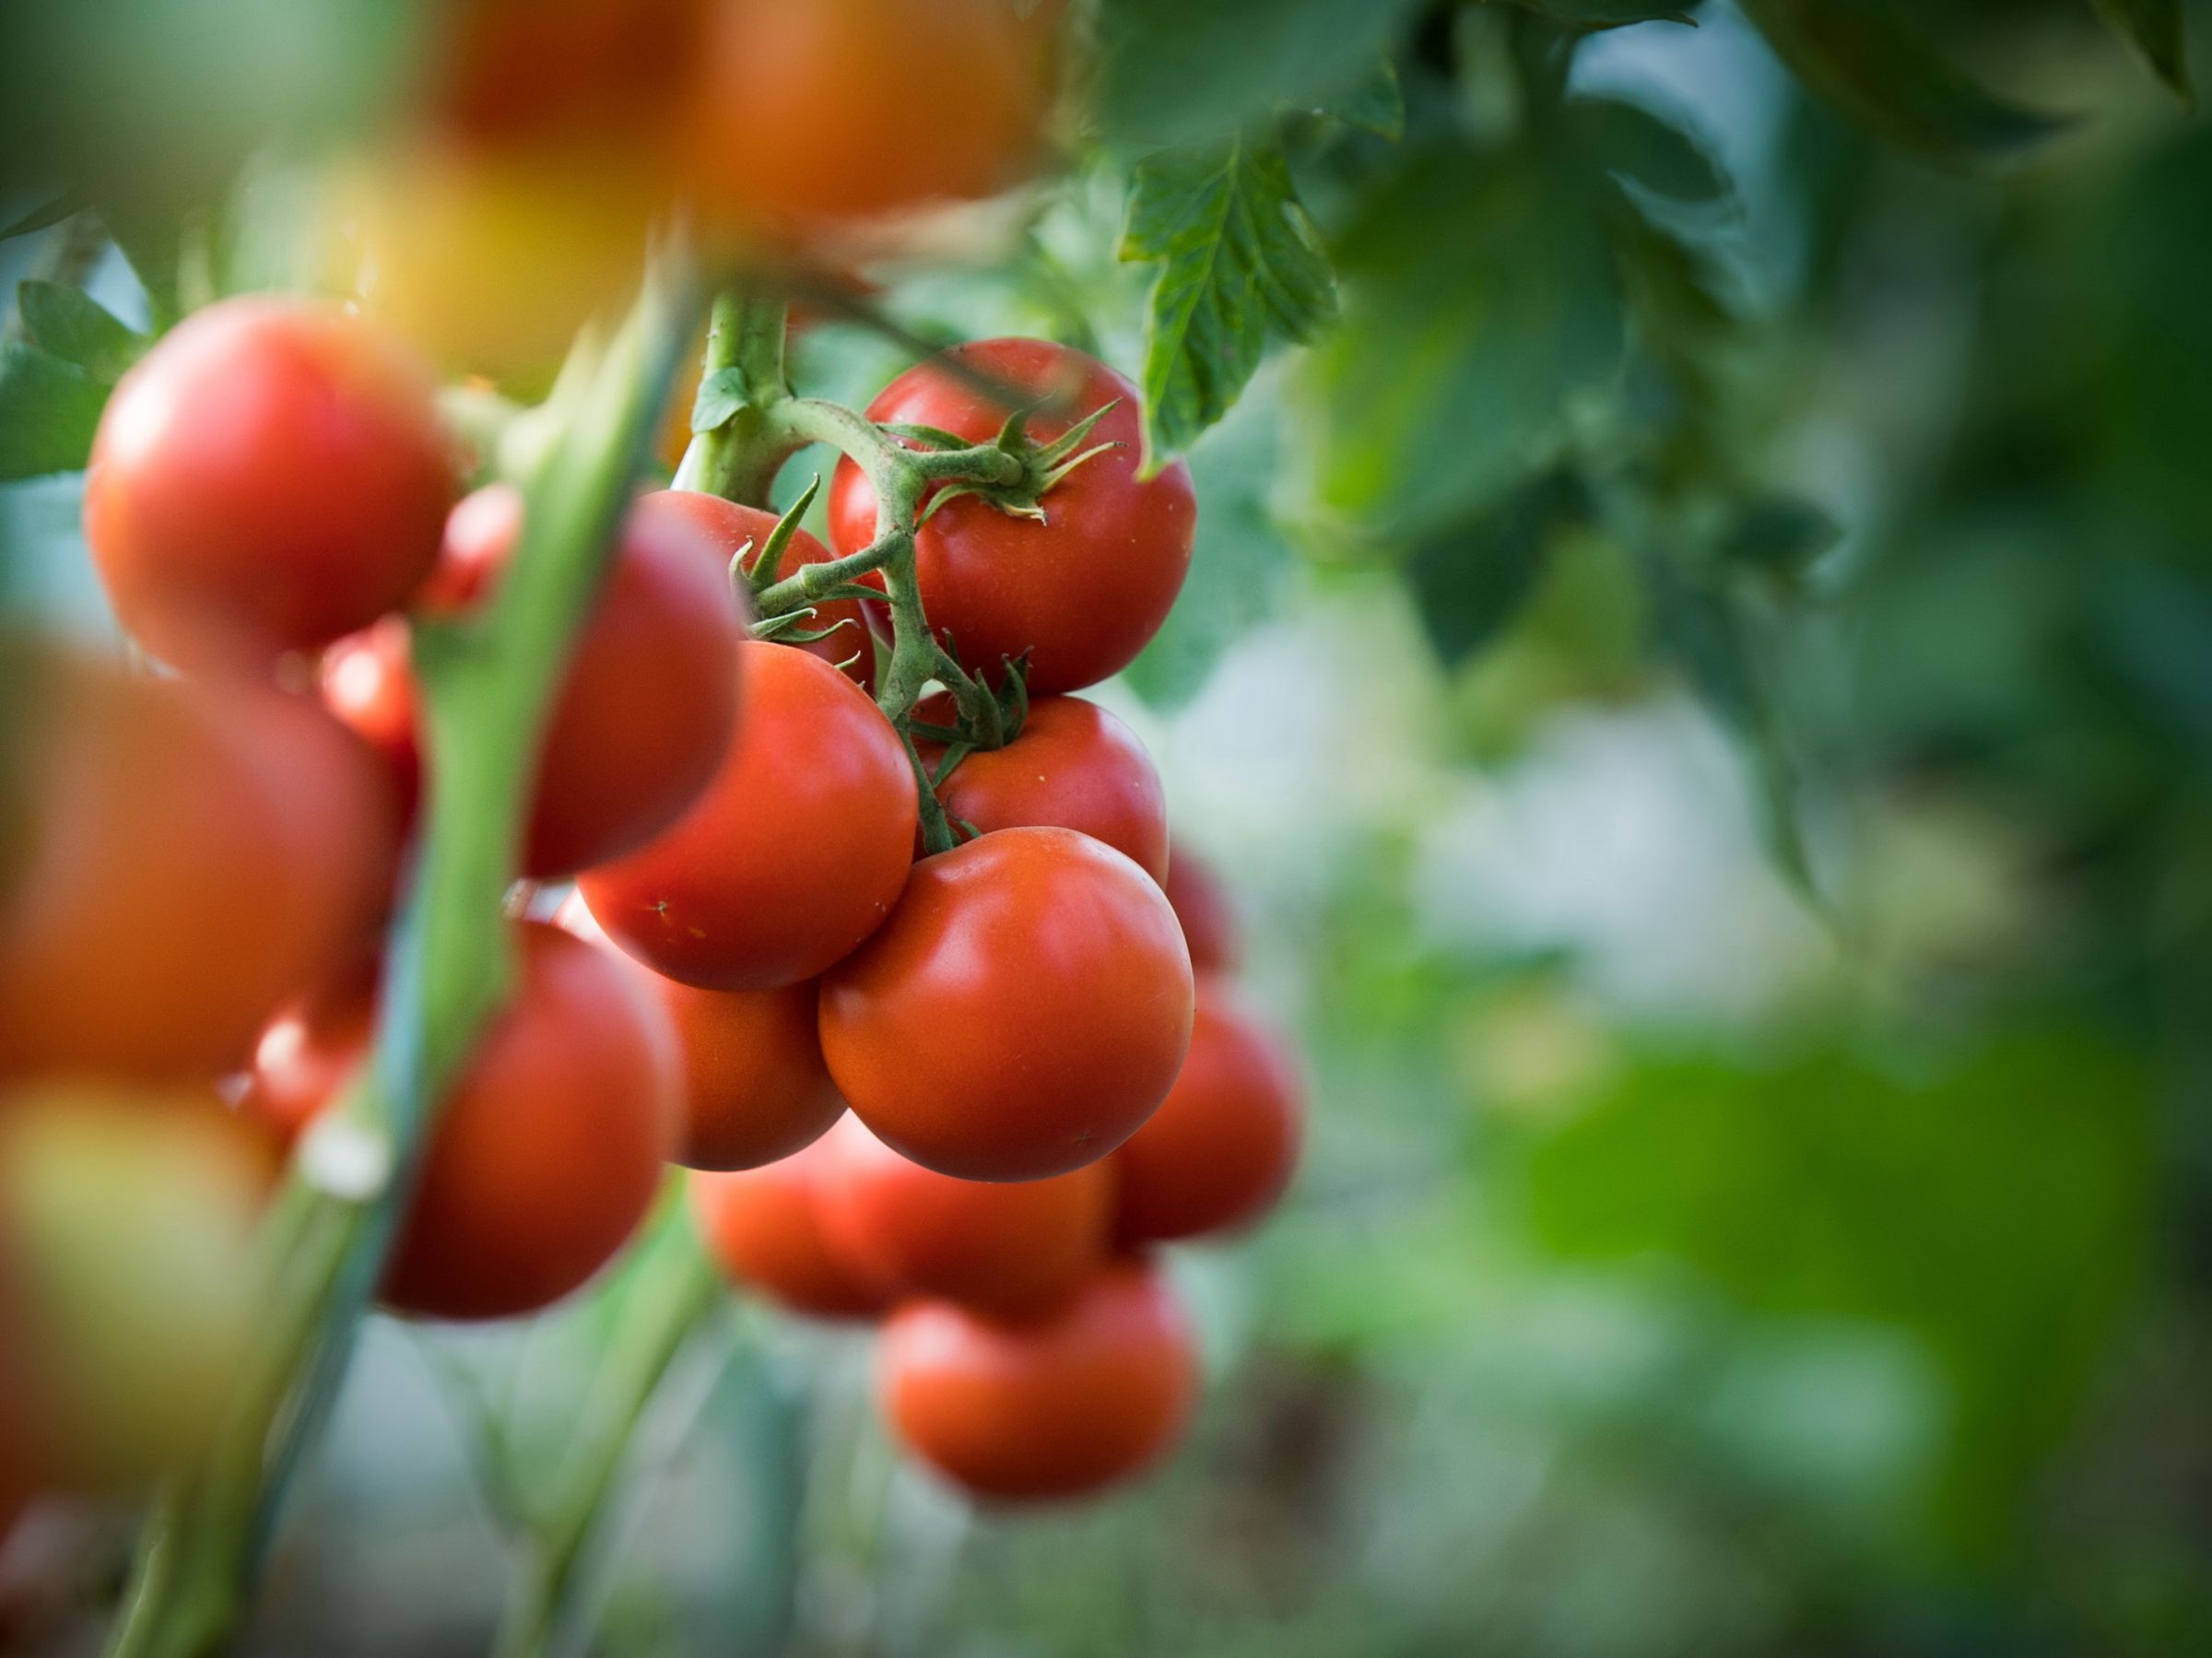
\includegraphics[width=0.6\linewidth]{saint_pierre.jpg}
			\caption{ Tomate de la variété Saint Pierre \protect\footnotemark.}
	        \label{tomate}
		\end{figure}
		\footnotetext{\href{https://www.jardiner-malin.fr/fiche/culture-tomate.html}{https://www.jardiner-malin.fr/ 
		fiche/culture-tomate.html}}
			  
La tomate appartenant à la famille des \textit{Solanaceae},
elle est apparentée à de nombreuses plantes  (poivron, pomme de terre, aubergine, tabac).
Ainsi dans une certaine mesure, les connaissances acquises grâce aux études menées sur la tomate peuvent être  appliquées à ces plantes.  Par ailleurs le cultivar Saint Pierre est utilisé en routine pour les élevages de nématodes à galles. La culture est donc maîtrisée et la durée du cycle de \textit{M. incognita} est connue pour cette plante.
Pour toutes ces raisons, la tomate est un excellent  modèle d'étude / matériel de recherche  pour la famille des \textit{Solanaceae}.
	
\subsubsection{Les nématodes}
	Les nématodes  utilisés dans cette étude proviennent d’une collection maintenue
	dans l'UMR ISA  (INRAE 1355 PACA, site de Sophia Antipolis; CNRS 7254; Université Côte d'Azur), dans le Sud-Est de la France. Cette
collection comprend environ 80 souches de \textit{Meloidogyne}, issues du monde entier,
représentatives des espèces les plus nuisibles. Une  souche
avirulente vis-à-vis du gène $Mi$-$1$ de la tomate a été utilisée dans cette étude. La souche \textit{M. incognita} Morelos  (espèce originaire du Mexique) a
été utilisée dans cette expérimentation  qui a pour but  de quantifier les dégâts que causent l'infestation de racines de tomates sensibles  par les nématodes.   
Pour les besoins de notre expérience nous avons au préalable produit une quantité abondante de nématodes \textit{M. incognita} (voir \Cref{secan1}). 
	
	
\subsubsection{Déroulement de l'expérience}
	Au début de l'expérience ($t=0$), nous avions à notre disposition $40$ plantes âgées de $42$ jours cultivées dans des  pots en plastique de dimension 9x9x9 cm  remplis d'un mélange de
sol stérilisé et sableux. La masse de sol dans chacun des $40$ pots   était de $470$ grammes.  
Ces plantes étaient maintenues dans une chambre climatique  en conditions contrôlées  à  
24$^{\circ}$ C, avec un éclairage artificiel ($16$ h de jour et 8 h de nuit) et une humidité relative de $60$ à $70$ \%.  L’arrosage était manuel. 
Les $32$ plus belles plantes ont été conservées pour l'essai.
Les densités de populations de nématodes initiales ($P_i$)  testées étaient de $0$; $0,6$; $8$ et
$16$  nématodes de stade J2 / g de sol (UN).   
Nous avons effectué huit réplicats par modalité d'inoculum et randomisé les positions des plantes sur le tablar.   En effet, bien que les plantes aient été placées en conditions contrôlées, des différences dans la taille des racines et des plants subsistent, pouvant entraîner des différences de mesures au sein de la même modalité d'inoculation, en interaction potentielle avec des effets de bordure, d'éclairage ou d'arrosage. En randomisant les plantes sur le tablar, ces effets étaient homogénéisés sur toutes les modalités. Les plantes  ont été récoltées  35 jours après inoculation afin d'évaluer l'effet des nématodes sur la croissance de la plante et de comparer nos données à celle de \citet{Ehwaeti1998}. Les plantes ont été repiquées dans des pots et des sols avec différentes densités de nématodes utilisés  en pièce climatique.  Nous présentons dans  \Cref{secan2} le protocole de quantification du nombre de nématodes dans la plante. 
	 
	\subsubsection{Les mesures d’intérêt} \label{mesures}
	 
	 De nombreux indices de notation existent afin d’évaluer l'infestation des plantes par les nématodes à galles. Les indices de galles (IG) \citep{Zeck1971} sont utilisés principalement sur le terrain lorsque plusieurs cycles de nématodes ont eu lieu. À partir d'indices de  galles des racines et  de 
 masses d’œufs ou taux de reproduction, \citet{Canto-Saenz1985} a classé la réponse des plantes aux nématodes à galles
comme sensibles (bonne reproduction des nématodes et apparitions  sévères de galles), tolérantes (bonne reproduction des nématodes et peu de galles)  ou résistantes (pas de galles).
Pour les tests en conditions contrôlées avec un taux d’inoculum déterminé et un seul cycle de développement (environ 35 jours à 24$^\circ$),  on compte  plutôt le nombre de pontes sur racines à l'aide d'une loupe, chaque ponte correspondant à une larve J2 ayant pénétré dans la racine. Pour réaliser le comptage, les masses d’œufs de \textit{Meloidogyne incognita}   sont colorées à l'éosine ($4,5$ g / l d'eau). La coloration confère une couleur rose très pâle à tout le système racinaire, les masses d’œufs prennent une coloration rouge plus foncée (\autoref{fig:p_m}).
	\begin{figure}
	    \centering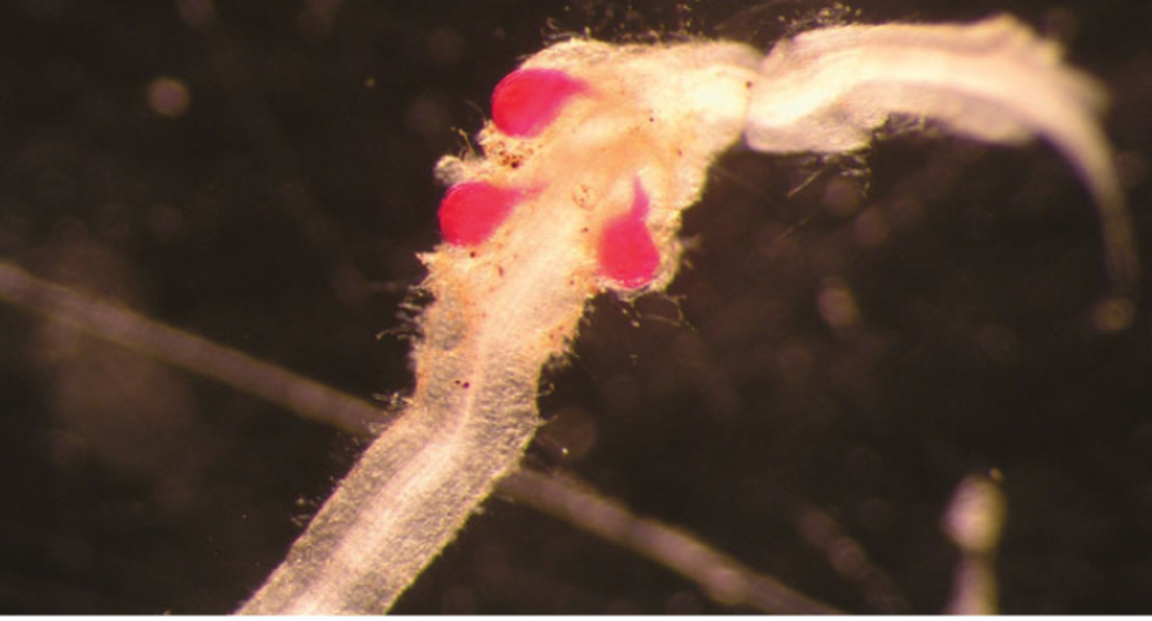
\includegraphics[width=0.6\linewidth]{ponte1} 
	   \caption[Observation des pontes  de \textit{M. incognita} après coloration à l'éosine des racines de tomate.]{Observation des pontes  de \textit{M. incognita} après coloration à l'éosine des racines de tomate. D'après \citet{Greco2010}.}
	   \label{fig:p_m}
	\end{figure}
	Ces mesures étant destructives, elles ont  été réalisées à la fin de l'expérience, soit $35$ jours après inoculation. Les masses fraîches des parties  racinaires ont également été mesurées. % Dans cette étude, comme pour l'expérience d'\citet{Ehwaeti1998}  nous allons considérer la biomasse racinaire relative c'est à dire la masse fraîche des parties racinaires avec infestation divisé par la masse fraîche des parties  racinaires sans infestation.
	La comparaison de nos données  avec celles des données de \citet{Ehwaeti1998} a  également été réalisée afin de comparer les deux expérimentations qui diffèrent par de nombreux facteurs. Il s'agit par exemple de la souche du nématode, de l'âge des plantes et la taille initiale des plans avant inoculation, des conditions d'éclairage ou d'arrosage lors du déroulement de l'expérience et des conditions pédologiques.
	
	
	
	\subsubsection{Analyses statistiques}
	Dans un premier temps nous nous sommes intéressés aux données brutes de l'expérience après inoculation (\textit{i.e.}  les mesures effectuées n'ont pas été transformées) :
\begin{itemize}
\item la première variable analysée est le nombre de nématodes final dans la plante après 35 jours de culture,
\item la seconde variable analysée est la masse fraîche  des parties racinaires après 35 jours de culture.
\end{itemize}
	%Nous avons effectué ces transformations pour comparer ces mesures avec l'expérience d' \citet{Ehwaeti1998} dans la sous section suivante.
	
	
	
	Pour déterminer  l'effet des densités initiales d'inoculum sur le nombre de nématodes final dans la plante et la masse fraîche  des parties racinaires, deux  \glspl{anova} à un facteur ont été conduites. La première  sur la variable  expliquée (\textit{i.e} variable dépendante) le nombre final de nématodes  dans les racines   en fonction des quatre modalités (témoin, faible, intermédiaire, élevée) du facteur de densités initiales de nématodes dans le sol. Un test de Fisher a été utilisé pour tester si au moins une des moyennes du nombre final de nématodes dans la plante était significativement différente des autres. 
La seconde a été conduite sur la variable expliquée  la masse fraîche  des parties racinaires  de tomates sensibles en fonction des  quatre modalités de densités initiales de nématodes considérés dans cette expérience.  
Enfin, des tests  de Tukey \gls{anova} (post-hoc)  ont aussi été conduits sur les analyses de variance afin d'évaluer la significativité des différences entre modalités comparées deux à deux.
	
	\subsubsection{Calibration du modèle}
	
	\iffalse
	Avant même le calcul de la meilleure estimation des paramètres inconnus de notre modèle grâce à nos données, nous nous sommes demandés comment notre modèle pouvait refléter les résultats de notre expérience dans une situation expérimentale différente \citep{Ehwaeti1998}. Pour rappel, l'étude de  \citet{Ehwaeti1998} traduit l’infection de plantes de tomates sensibles  ($cv.$ $ Moneymaker$)  par des nématodes
avirulents du genre \textit{M. incognita}. Il s’agit de quatre jeux de données expérimentales reliant la densité initiale de nématodes dans le
sol (0 ; 0,03 ; 0,16 ; 0,8 ; 4 ; 20 J2 / g de sol) à leur densité finale dans la plante à la fin de 42 jours et 135 jours  de culture. La biomasse racinaire relative (\textit{i.e.}, la biomasse racinaire
divisée par la biomasse racinaire témoin sans nématode) était également
mesurée. À partir des données à 135 jours nous avons pu estimer   $x$ le facteur de conversion entre masse de racine et de site nourricier, $\beta$ le taux de contamination, $k$ le facteur de modulation de la croissance racinaire  et $y$ la masse d'une galle par rapport à un tissu sain. Les autres paramètres du modèle sont donnés par la littérature. 
Le paramètre $\beta$ qui représente le taux de contamination de l’hôte par le parasite est un  paramètre qui influence  fortement les sorties du modèle.  Nous supposons que ce taux serait plus sujet à des variations puisque nous avons mesuré des densités de nématodes finales dans la racine différentes aux données de  \citet{Ehwaeti1998}. Par ailleurs,
nous pouvons supposer que la valeur du paramètre $y$ qui contrôle la masse des galles soit plus élevée dans le cadre de notre expérimentation puisque la biomasse racinaire relative en moyenne était supérieure à 1 dans notre expérimentation.
	\fi
	
	Les mesures  de notre  expérimentation à 35 jours ont été utilisées pour calibrer notre modèle.
Nous voulions déterminer la meilleure estimation des valeurs des paramètres $x$, $\beta$, $k$, et $y$  grâce à l'ajustement du modèle  à nos données expérimentales.
Pour ce faire, la première étape de la calibration  a consisté à  transformer les données brutes émanant de notre expérimentation. Le lien qui existe entre les variables mesurées et celles considérées pour la calibration est le suivant : 
\begin{itemize}
\item  la variable nombre final de nématodes dans la plante  après 35 jours de culture a été transformée en une nouvelle  variable, la densité finale de nématodes  dans la plante  après 35 jours de culture (la nouvelle unité : nem / g de sol),
\item  la variable  masse fraîche  des parties racinaires  a été transformée en une nouvelle  variable, la biomasse racinaire relative qui correspond à la masse fraîche  des parties racinaires avec infestation divisée par la masse fraîche des parties racinaires sans infestation.
\end{itemize}
	
	Dans le cadre de notre expérience nous ne disposions pas de la valeur du paramètre $ H_0 $ : la masse initiale de racine d'une plante âgée de 42 jours~\footnote{car nous n'avons pas réalisé cette expérience}.   Par conséquent, la seconde étape de la procédure de calibration a consisté à obtenir cette valeur. 
Nous avons estimé la valeur de biomasse racinaire d'une plante de 42 jours à partir du modèle proposé par \citep{Leskovar1990}.
	
	\iffalse
	\begin{equation}
	H_0^{42}= H_0 + \mu t  \quad \text{pour } t = 42,  H_0=H_0x,
	\label{eq:H0}
	\end{equation}
\noindent dans laquelle $H_0$ est la  biomasse racinaire initiale d'une plante à $t=30$ jours  et $\mu$ la croissance racinaire en milligrammes par jour . 
	\fi
	%Les différences entre deux expérimentations peuvent être fréquentes notamment  à causes des conditions expérimentales qui diffèrent les une des autres : (i) l’espèce et l’âge  des plantes avant l'inoculation, (ii) la souche  de nématode. 
	 
	
	La troisième  étape a consisté en utilisant la même méthode de calibration  détaillée dans~\Cref{MethodsS2} du manuscrit pour les données \citet{Ehwaeti1998} à estimer les nouvelles valeurs pour les paramètres $x$, $\beta$, $k$ et $y$  en procédant à l'ajustement du modèle  cette fois-ci  pour  nos propres données expérimentales. 
Les valeurs des paramètres $\beta$, $x$, $k$ et $y$ ont donc été obtenues par ajustement du modèle 
\eqref{sys0} du \autoref{chapter_3} à l'ensemble des données expérimentales issues de notre expérience allant jusqu'à 35 jours de culture.  Pour obtenir cette estimation nous avons retenu  les valeurs de paramètres qui minimisent la distance entre la sortie du modèle et les données.  Nous avons testé plus de 1000 itérations de la fonction optim() grâce à une parallélisation \footnote{à l'aide du package snow (\href{https://CRAN.R-project.org/package=snow}{https://CRAN.R-project.org/package=snow}) de R} du code et pour des conditions initiales différentes.
	%Enfin, par ces différentes étapes nous avons pu identifier dans quelle mesure les valeurs de paramètres diffèrent les unes des autres en fonction des deux expérimentations et l'implication de ces différences en général :
	
	%\begin{enumerate}[label=\roman*., itemsep=7pt, topsep=5pt]
	%\item   pour le choix de la variation autour des  valeurs de référence des paramètres pour comprendre l'effet de chaque paramètre du modèle PHEI sur les sorties du modèle,
	%\item  pour  obtenir des scénarios épidémiologiques des plus réalistes et pertinents que possible,
	%\item pour étudier la robustesse des stratégies.
	%\end{enumerate}
	
	
	
\subsection{Résultats et Discussion} \label{sec:résultats-chapitre4}
	
	
	%\subsection*{Analyse de sensibilité sur la sortie rendement des sensibles}
	%\subsection*{Effet des coûts de fitness sur la durabilité, le gain et le ratio en fonction de beta et r}
	%\subsection*{Effet des coûts de fitness sur la durabilité, le gain et le ratio en fonction de la mutation}
	
\subsubsection{Effet de la densité initiale de nématodes dans le sol sur les données brutes de l'expérience}
	
	Deux jeux de données expérimentales ont été obtenus dans cette étude. Le premier jeu de données correspond  au nombre de nématodes par  plante à la fin de $35$ jours de culture en fonction de quatre valeurs de densités  initiales de nématodes (\autoref{tab:nem_root}). Le second jeu de données correspond à la   masse racinaire  après $35$ jours de culture selon les quatre modalités de  densités initiales de nématodes (\autoref{tab:nem_root}).  Selon nos résultats, la variation dans les moyennes du nombre de nématodes  après 35 jours, de 32 plantes inoculées avec 3 densités initiales de nématodes différentes et 8 plantes non-inoculées témoins n'est pas due au hasard, $i.e.$ on observe bien un \og effet densité initiale de nématodes significatif \fg{}  ( \textit{p-value} $=$ 5,654 $\times$ $10^{-10}$, test de Fisher). Nous observons également cet effet significatif de la variation dans les moyennes  de masse fraîche racinaire en fonction des 4 modalité de densités initiales de nématodes (\textit{p-value} $=$ $0.0006199$, test de Fisher).
	
	 	\begin{figure} 
		  \centering
			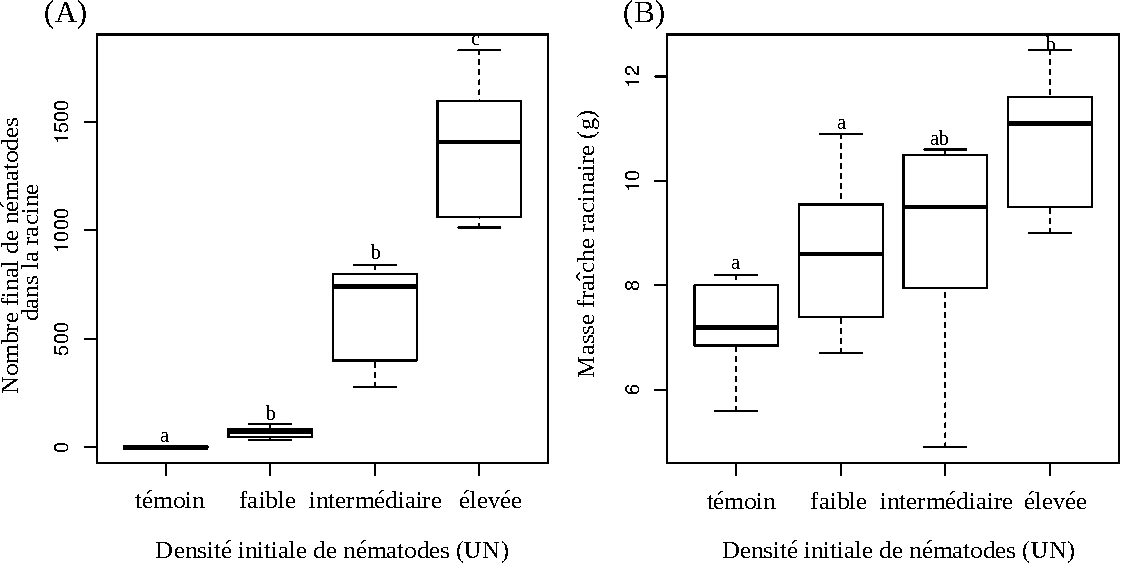
\includegraphics[width=1\linewidth]{boxplot_donnee_brute.pdf}
			\caption[Effet de la densité initiale de nématodes sur A) le nombre final de nématodes dans la racine et B) 
			la masse fraîche racinaire.]{. Box plots (A)   du nombre  final de nématodes dans la racine et (B)   des 
			masses fraîches racinaires après 35 jours de culture,  en fonction des densités initiales de nématodes dans 
		    le sol. Par convention, si deux moyennes partagent une même lettre (en minuscule) elles ne  sont pas 
            significativement différentes. En revanche, si deux moyennes ne partagent pas une même lettre alors elles   
            sont significativement différentes   (tests bilatéraux de Tukey pour un risque d’erreur de première espèce 
            $\alpha$ = $0,05$). } 
			\label{dens_bio}
		\end{figure}
		
	
	En premier lieu, on constate que  le nombre de nématodes dans la plante après $35$ jours de culture augmente avec la densité initiale de nématodes dans le sol	(\autoref{tab:nem_root}).
La plus forte valeur de nombre de nématodes dans la plante est de   $1830$ pour une densité initiale de nématodes de $16$  J2 / g de sol. %une quantité initiale de nématodes égale à 11 568 
	  D’après l'analyse de variance et  le test de Tuckey, nous avons observé  un nombre de nématode en moyenne  significativement (\textit{p-value} $< 0,05$)  différent entre la modalité de densité initiale élevée et  les autres modalités (\autoref{dens_bio}A). Par exemple, la moyenne du nombre final de nématodes  dans la plante pour une densité initiale de nématodes de $16$ J2 / g de sol était de 1372, contre une moyenne de 69 nématodes dans la plante pour une densité initiale de nématodes de 0,6 J2 /g de sol. De même, une dose d'inoculation de 8 J2 / g de sol (intermédiaire) était statistiquement différentes  des  modalités témoin et élevée (\textit{p-value} $< 0,05$). Une dose d'inoculation faible  était statistiquement semblable à une dose intermédiaire (\textit{p-value} $> 0,05$).  Ce test a permis de mettre en évidence qu'il existe bien des différence significatives entre quasiment toutes les modalités d'inoculation utilisées dans cette expérience. 
	    
	En second lieu, nous avons observé une augmentation de la masse fraîche racinaire après $35$ jours de culture lorsque  la densité initiale de nématodes dans le sol augmentait (\autoref{tab:nem_root}). La plus forte  valeur  de masse fraîche racinaire est de $12,5$ g pour la valeur la plus forte  d'inoculum initial (\textit{i.e.} 16 J2 / g de sol). La valeur moyenne de masses racinaires était de $10,7$ g toujours pour cette valeur d'inoculum initial. À titre de comparaison la masse fraîche racinaire pour le témoin non inoculé était de 7,2 g en moyenne.
	 D’après la seconde analyse de variance et  le test de Tukey, nous avons observé que cette différence de masse fraîche racinaire   entre la modalité de densité initiale élevée et  celle du  témoin non inoculé est statistiquement significative (\textit{p-value} $< 0,05$)  (\autoref{dens_bio}B).  En revanche, les deux autres modalités (faible et intermédiaire) étaient statistiquement semblables (\textit{p-value} $> 0,05$) au témoin non inoculé.  La différence observée serait potentiellement liée à la masse des galles. Cet effet semble assez marqué et sera pris en compte lors de la comparaison de notre expérience avec celle de \citet{Ehwaeti1998}. 
	 
	
	\begin{table}[ht]
	\centering
	\caption{  Masse d’œufs et  masse des parties racinaires en  moyenne  $\pm$ (SD)$^1$   par plante en fonction de $P_i$ (35 jours après inoculation).}
	  \begin{tabular}{lccc}
	\hline
	$P_i$ J2 / g de sol  & nombre total de nématodes / plante    &    masse racinaire (g) / plante  \\ \hline 	 
	0 (témoin)           & 0                                     &     7,2 $\pm$ (0,87)                                        \\
	0,6  (faible)                                                & 68,7 $\pm$ (25,8) &  8,6 $\pm$ (1,46)                                               \\
	8    (intermédiaire) & 624,9  $\pm$ (232)                    &  8,9 $\pm$ (2,00)                                      
\\
	16 (élevée)                                                  & 1371,7  $\pm$ (306)    &     10,7 $\pm$ (1,29)                                     \\ \hline
	\end{tabular}
	\label{tab:nem_root}
	  \par\medskip\footnotesize
	 ${}^1$moyenne des 8 réplicats par inoculum et  l'écart type (SD)
	\end{table}
	\subsubsection{Comparaison avec l'expérience de \citet{Ehwaeti1998}}
	 La première étape de la comparaison des deux expérimentations a consisté à  transformer les données brutes émanant de notre expérimentation pour comparer ces données transformées avec celles  de \citet{Ehwaeti1998}. La seconde étape a été de décrire, relever et analyser les principales différences entre les deux expérimentations. La dernière étape a consisté à proposer des explications  pouvant expliquer les différences de mesures identifiées.
	 
	 
	    \begin{figure}[H] \centering
		    	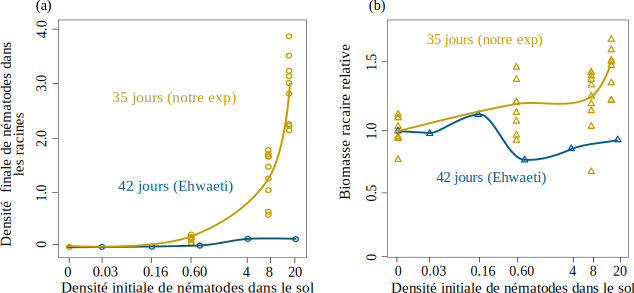
\includegraphics[width=1\linewidth]{Ehwaeti1998_nousExp}
			    	\caption[Comparaison des (a) densité finale de nématodes dans les racines et (b) biomasse racinaire 
			    	relative en 
			    	fonction de la densité initiale des nématodes dans le
		        le sol.]{ (a) Densité finale de nématodes dans les racines et (b) biomasse racinaire relative après 35 
		        jours  
		        (en or) et 42 jours (en bleu), en fonction de la densité initiale des nématodes dans le
		        le sol (échelle logarithmique). Les traits bleus relient les valeurs moyennes expérimentales issues de  
		        \citep{Ehwaeti1998}.  Les traits or relient les valeurs moyennes expérimentales issues de notre 
		        expérience.}
		    	\label{comp:exp}
	    \end{figure}
	    
	La figure \ref{comp:exp}a montre les données expérimentales de densités de nématodes dans la plante après 35 jours de culture (notre expérience) et 42 jours de culture  \citep{Ehwaeti1998} en fonction des densités initiales de nématodes dans le sol pour les deux expérimentations. 
En ce qui concerne nos données expérimentales, nous pouvons observer des densités de nématodes plus importantes dans la plante à 35 jours qu'à 42 jours,  en particulier pour de fortes populations initiales de nématodes (8, 16 et 20  nématodes par gramme de sol). Ceci peut s'expliquer par de nombreux facteurs (différence entre âges des plantes, cultivars, souches de nématodes) que nous allons aborder plus longuement par la suite \citep{Windham1986, Barker1991, McSorley1992}. 
	
	
	La   \autoref{comp:exp}b illustre les données de biomasse relative  en fonction de la densité initiale de nématodes dans le sol, après  35 et 42  jours de culture pour les deux expérimentations.
On observe que les données  de biomasse relative à 35 jours sont plus élevées
que celles à 42 jours, en particulier pour les fortes infestations initiales (8 et 16  nématodes par g
de sol). Tout d'abord, dans le cadre de notre expérience, nous avons  observé des biomasses racinaires relatives supérieures à 1 contrastant avec les données à 42 jours où les biomasses racinaires relatives étaient  proches de 1. Cela peut donc indiquer  que l’infestation avait peu d’impact sur la plante à ce stade dans l'expérimentation de \citet{Ehwaeti1998} par rapport à notre expérience. 
Une  mesure où la biomasse relative est supérieure à 1 est une mesure où la biomasse racinaire avec infestation est supérieure à la biomasse racinaire sans infection. L'explication la plus plausible est que la biomasse racinaire avec infestation est composée également de galles et de masses d’œufs qui sont des caractéristiques symptomatiques de l'infection par des nématodes (voir section \ref{contournement} du chapitre \ref{intro}). Par conséquent,
on peut en déduire que la masse  des galles et de masses d’œufs  était  donc beaucoup plus importante dans notre expérimentation que dans l'expérience de \citet{Ehwaeti1998}. 
	
	Un des points intéressants à noter à l'issue de  notre expérience  était que nous n'avons pas observé de perte de biomasse racinaire (i.e biomasses racinaires relatives inférieures à 1) avec l'augmentation de la densité initiale. Au contraire, plus l'infestation initiale était forte  plus la biomasse racinaire relative était grande. Ce résultat peut paraître contre intuitif en particulier pour les fortes infestations.    L'explication pour laquelle nous n'avons pas observé de perte  de masse  racinaire  à haute densité de nématode est  due potentiellement au temps d'observation post-infection.  La perte de masse racinaire pour de fortes infestations en moyenne n'était pas observable car  probablement compensée par cette masse de galles qui résultent de l'infection.  Pour une
durée où l'épidémie est courte (i.e une durée d'observation à 35 jours),  la plante peut pousser  et ainsi la population de nématodes peut se développer. À ce stade d'observation on conclut plutôt que l'augmentation de la densité initiale dans le sol a  comme effet d'augmenter la présence et la masse de galles  plutôt qu'une éventuelle observation d'une perte de biomasse racinaire liée en général à un fort impact de l'infection par les nématodes sur la croissance racinaire  \citep{Ehwaeti1998}.  
	
	 À titre de comparaison
	dans l'expérience de \citet{Ehwaeti1998} cette fois-ci conduite  jusqu'à 135 jours et pour de faibles densités de nématodes  (0,03; 0,16  nématodes par g de sol) (voir \autoref{fig2} du~\autoref{chapter_3}), nous avions aussi observé des valeurs de biomasse racinaire relative supérieures à 1. Dans ce cas de figure,
l'infection étant faible au début, la plante peut pousser  et ainsi la population de nématodes peut se développer. Comme dans le cadre de notre expérience, l'apparition des galles et de pontes en interaction avec la croissance racinaire conduit à des biomasses racinaires élevées (\textit{i.e.} supérieures à 1).  En revanche, nous avions observé une biomasse relative faible pour de fortes populations initiales de nématodes (4 et 20 nématodes par g de sol). Ainsi, on peut imaginer que la croissance de la plante ait été fortement impactée durant la saison de culture d'une durée de 135 jours. De surcroît, on peut supposer que de faibles biomasses relatives  aurait été plus visibles si nous avions conduit notre expérience plus loin dans le temps.
	
			
	
	\begin{table}[ht]
	  \centering
	      \small
	  {\renewcommand{\arraystretch}{1.2}
	  \caption{Comparaison des protocoles expérimentaux entre  notre expérience  et celle de  \citet{Ehwaeti1998} . }
	
	  \begin{tabular}{llll}
	\hline
	                      &  Ehwaeti et \textit{al} & Nous            & Unités \\ \hline
	Variété des plantes & Moneymaker & Saint Pierre & --\\
	Âges des plantes    & 30                                          & 42 & jours                      \\
	Origine souche      & ?                                           & Morelos &  --                    \\
	Température         & 24          & 24  & degrés Celsius                     \\ 
	Durée de la culture & 42 et 135                                   & 35 & jours                      \\ 
	Densités initiales de nématodes  & 0; 0,03; 0,16; 0,8; 4; 20  &  0; 0,6; 8; 16  & J2 / g de sol \\
	Dimension des pots    & 5,4                                       & 0,7                     & $dm^3$ \\ 
	Masse de sol          & 3650                                      & 470 & g \\ \hline
	\end{tabular}
	
	\label{tab:comp:exp}}
	\end{table}
		
	
	En conclusion, ces différences de mesures entre les deux expériences à 35 jours et 42 jours pourraient s'expliquer par de nombreux facteurs  (\autoref{tab:comp:exp}). Par exemple,  l'âge des plantes avant inoculation peut influencer l'épiderme des racines et la taille du chevelu racinaire. Dans l'expérience de \citet{Ehwaeti1998}, les auteurs ont infesté les pots avec différentes modalités d'inoculation pour des plans âgés d'environ 30 jours (plants de tomates avec deux  feuilles). Dans notre expérience, les plantes de tomates étaient âgées de 42 jours (plants de tomates de 5 à 6 feuilles). Ainsi nous pouvons supposer que le chevelu racinaire était plus important.
Par ailleurs, la souche de nématodes est  également source de variabilité, particulièrement  pour des composantes comme la capacité migratoire, le succès de l'infection, le taux de contamination, la mortalité du nématode et  la reproduction du nématode \citep{Pegard2005, Castagnone-Sereno2007, Djian-Caporalino2011}.
Par conséquent, ces différences justifient l'étude de différents scénarios épidémiologiques  dans le but de déterminer des stratégies optimales de rotations entres plantes résistantes et sensibles dans des conditions variées et leur robustesse (voir~\autoref{chapter_3}).  
	
	
	Dans la suite, nous avons cherché à savoir si notre modèle était capable de refléter les données expérimentales de notre expérience dont nous avons pu observer une  différence notable avec les données de \citet{Ehwaeti1998}. 
	 
\subsubsection{Calibration du modèle à nos données expérimentales}   \label{sec:calibration}

	 \begin{figure}[H]
			\centering
				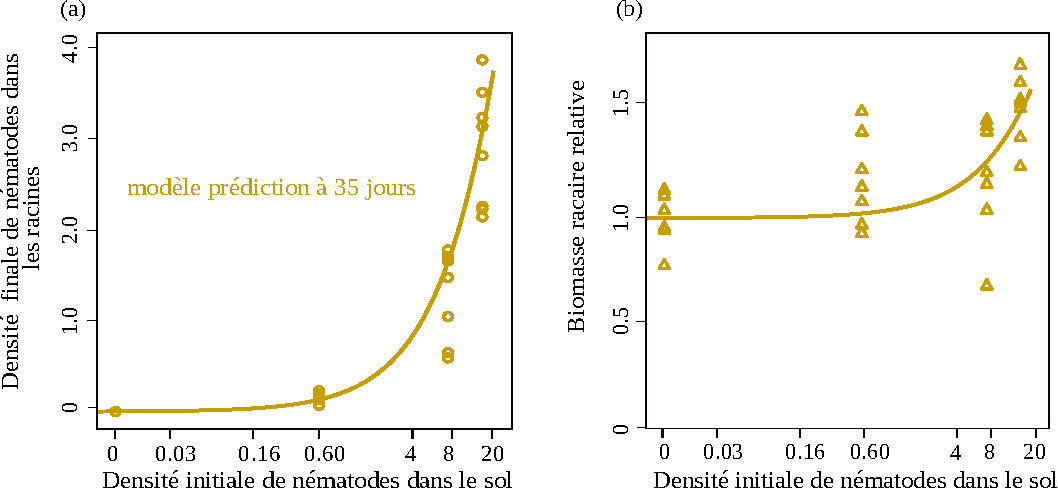
\includegraphics[width=1\linewidth]{fit_exp.pdf}
				\caption[Ajustement du modèle aux données issues de notre expérience]{Ajustement du modèle aux données 
				issues de notre expérience. (a) Densité finale de nématodes dans les racines et (b)  biomasse racinaire 
				relative après 35 jours de culture, en fonction de la densité initiale de nématodes dans le sol 
				(échelle logarithmique). Les sorties du modèle sont représentées par des courbes pleines, les cercles 
				et les triangles représentent des mesures expérimentales.}
			    \label{fit:expe} 
		\end{figure}
		
	 
	    
	 La meilleure estimation des paramètres du modèle par rapport à nos données expérimentales a été retenue.
L'ajustement  a permis de reproduire  fidèlement la densité finale de nématodes  dans les racines et la biomasse racinaire, en fonction des densités initiales  de nématodes dans le sol (\autoref{fit:expe}).   
L'estimation de seulement 4 paramètres parmi 15 autres nous a permis d'obtenir un tel résultat. 
	 
	 D'autre part, compte tenu des  différences notables entre notre expérience et celle de \citet{Ehwaeti1998}, le fait que notre modèle soit capable de refléter à la fois  les données expérimentales des deux expérimentations est remarquable.  Cela indique que notre modèle peut très bien s'adapter à différentes situations épidémiologiques. Notre modèle peut prendre en compte différentes situations  en tenant compte de  de la souche du nématode  et de la plante étudiées par réajustement du paramètre $\beta$, $x$ et $y$. Ces paramètres sont donc cruciaux pour un bon ajustement du modèle aux données expérimentales sachant les autres valeurs de paramètres depuis la littérature. De plus ces paramètres estimés ont une très forte interprétation biologique. 
	 
	\subsubsection{Comparaison des valeurs de paramètres obtenues entre les deux expériences}
	 
	 La comparaison entre les valeurs de paramètres estimés  à partir de l'ajustement du modèle aux données expérimentales de notre expérience  et celles de \citet{Ehwaeti1998} est donnée dans le \autoref{comp:para}. 
Le paramètre $\beta$ qui représente le taux de contamination de l’hôte par le parasite est un  paramètre qui influence  fortement les sorties du modèle. 
Sous l’hypothèse d'une répartition aléatoire et homogène des nématodes et des racines dans le sol, la probabilité qu’un site nourricier d’une racine saine $H$ soit infecté entre un temps $t$ et un temps $t+dt$ est proportionnel
à la fréquence des nématodes dans le sol et donc à leur densité $P$. Le nombre total d’infections entre $t$
et $t+dt$ est égal à la probabilité qu’un site nourricier soit infecté multiplié par le nombre total de sites nourriciers, et est donc proportionnel à $PH$,  la constante de proportionnalité étant déterminée par le
taux de rencontre entre les racines et les nématodes. Nous supposons que ce taux serait plus sujet à des variations puisque nous avons mesuré des densités finales de nématodes  dans la racine élevées comparé à celles de  \citep{Ehwaeti1998}. Il dépend de manière implicite du taux de pénétration, du taux de contact, de l'efficacité de l'infection qui sont des paramètres variables selon les études expérimentales à cause de la composition du sol, de la souche du nématode et de la taille des racines différentes d'une expérience à l'autre. D'après nos résultats, le taux de variation entre la valeur du paramètre $\beta$ suite à l'ajustement à nos données ($\beta = 7\,10^{-5}$) et celle obtenue avec les données d'Ehwaeti ($\beta = 1.11\,10^{-4}$) est de l'ordre de  30\%.
Ce taux de variation est en accord avec le (ou les) niveau(x) de variation choisi(s) pour l'analyse de sensibilité, la définition des scénarios et l'étude de la robustesse (variations de $\pm 10 \%$, $20 \%$ et $30\%$ autour du scénario de référence) dans le \autoref{article}.  
	
\begin{table}[ht]
	\caption{Comparaison entre les valeurs des  paramètres ajustées à partir de nos données  expérimentales  et  à   
	partir des données de  \citet{Ehwaeti1998}.}
	\small
	{\renewcommand{\arraystretch}{1.5}
	%\begin{tabular}{lp{.3\linewidth}lcl}
	\begin{tabularx}{\linewidth}{lXlll}
	\hline
	Symbole & Description      &\multicolumn{2}{c}{Valeur(s)} & Unité \\
	&       & \multicolumn{1}{c}{Nous} & \multicolumn{1}{c}{Ehwaeti et \textit{al}} &   \\ \hline
	$H_0$   & Biomasse racinaire initiale                    &2760       & 1500    &   mg\\
	$\boldsymbol{x}$  &  Facteur de conversion entre masse de racine et densité de sites nourriciers & $ 1,13\,10^{-2}$      
	&  $4\,10^{-3}$   &   UR $\times$ mg de racines$^{-1}$ \\
	$y$     & Facteur de modulation de la masse des galles     & $15 $        & $4,2$ & --   \\
	$\boldsymbol{\beta}$ & Taux d'infection   & $7\,10^{-5}$   & $1,11\,10^{-4}$ & UR$^{-1}$ $\times$ jour$^{-1}$ \\
    $k$     & Facteur de modulation de la croissance racinaire &  $10,23$     &  $10,33$ &  -- \\ \hline
	\end{tabularx}
	}
	UR: nombre de sites nourriciers par gramme de sol.\\
	Les autres valeurs de paramètres sont données \autoref{table1} du~\autoref{chapter_3}.
	
	   \label{comp:para}
\end{table}
	
	
	 Dans notre étude, nous estimons que la masse relative  d'une galle par rapport à un tissu sain ($y$) pour une durée de culture à t=35 jours  est égale à 15, contre 4 pour l'expérimentation de \citet{Ehwaeti1998}, à t = 135 jours. Cette différence s'explique vraisemblablement par le fait que la masse des galles en moyenne dans notre expérience  à 35 jours soit  plus importante que l'expérience de \citet{Ehwaeti1998} à 135 jours où la présence de masse d’œufs en moyenne est moins importante car les cycles se chevauchent et que pratiquement tous les œufs ont éclos. À 35 jours de culture, la fin d'un cycle,  c'est le moment où les  femelles dans la galle et les masses d’œufs à l’extérieur de la racine sont les plus visibles et en grande  quantité, ainsi la galle est susceptible d’atteindre sa masse critique à cette durée d'observation alors que l'inverse se produit à 135 jours. Une autre explication de la différefattnce entre les valeurs de $y$  serait liée au fait que la masse de racine à 35 jours et celle à 135 sont différentes. Une racine à 135 jours de culture est beaucoup plus grosse qu'une racine à 35 jours de culture. Par conséquent, le poids relatif d'une galle par rapport à une racine de taille plus importante  peut conduire à une plus faible valeur de $y$. Inversement si le poids de la racine est faible cela peut conduire à une valeur de $y$ plus élevée.
	 
	 Enfin, nous avons observé que la valeur du paramètre $x$ dans notre expérience est 10 fois plus élevée que celle de \citet{Ehwaeti1998}. D'après nos hypothèses de modélisation cela  signifie que dans notre expérience le nématode  a besoin d'une quantité de racine 10 fois supérieure  à celle de l'expérience de \citet{Ehwaeti1998} pour constituer un site nourricier. De manière biologique cela reflète la prise en compte des différences intrinsèques qui subsistent  lors du parasitisme  des nématodes d'une plante à l'autre ou d'une racine à l'autre.
	
	\subsubsection{Conclusion} 
	 L’ajustement des paramètres de notre modèle sur les données expérimentales à 35 jours a permis de
reproduire assez fidèlement la croissance de la plante infectée par des nématodes au cours d’une saison de
culture.  Cette étude permet dans une certaine mesure de montrer que notre modèle mécaniste est suffisamment souple pour représenter des réalités expérimentales très différentes au prix de réajustements des valeurs des paramètres  puisque nous avons pu reproduire assez fidèlement deux expérimentations différentes. Cela signifie qu'à partir de notre démarche de modélisation nous pourrions simuler différentes situations épidémiologiques afin  de proposer les meilleures prédictions possibles et recommandations aux agriculteurs en fonction de la situation épidémiologique de leurs parcelles. Cette étude montre également que les valeurs de paramètres de référence   de notre modèle sont assez robustes puisque les nouvelles valeurs de paramètres estimés obtenues à l'issue de la calibration sont assez proches des valeurs de paramètres trouvées pour l'estimation avec les données de \citet{Ehwaeti1998}. 
	
\section{ Estimation de la survie des nématodes à l'intersaison en conditions de culture} 
	
	La démarche de modélisation que nous avons proposée dans ce projet de thèse nous a conduit à obtenir la valeur de tous les paramètres intrasaison  grâce à la littérature ou  par ajustement du modèle à des données expérimentales. Toutefois, nous ne disposions pas dans la littérature récente  la valeur   du paramètre $\varphi$, c'est-à-dire  la probabilité de survie du nématode à l'intersaison pendant l'hiver et en présence de culture.
Durant ma thèse, le but de notre travail a été d'estimer ce paramètre du modèle complet  (voir \eqref{sys1} et \autoref{figS1}).
Nous nous sommes donc intéressés à des données pluriannuelles de densité  de nématodes dans le sol en présence de cultures  habituellement plantées (\textit{e.g.} laitue batavia ou mâche) pendant l'hiver et en rotation avec des cultures  sensibles ou résistantes (\textit{e.g.} melon ou tomates) pendant le printemps. Ces données nous ont permis d’extrapoler une survie du nématode en présence de culture pour une durée adaptée  à notre intersaison hivernale. Ce travail a permis d’obtenir une modélisation plus réaliste du pathosystème \textit{Meloidogyne}-tomate sur le long terme.
	
	Pour traiter cet enjeu,  nous nous sommes  appuyés sur les données pluriannuelles d'un projet nommé \gls{GEDUNEM}  qui cherche à identifier de nouveaux leviers d'action dans les \og systèmes \fg{} de culture maraîchère afin d'améliorer l'efficacité et la durabilité des résistances aux nématodes. 
Ce projet d'une durée de 4 ans (2012-2016) a permis d'étudier l'impact de trois systèmes maraîchers sous abris combinant des rotations de cultures hôtes  et diverses pratiques agronomiques  (culture de plantes pièges, plantes biofumigantes et  solarisation (voir section \ref{lutte} du \autoref{intro}) pour augmenter l’efficacité du contrôle des nématodes et la durabilité des méthodes de lutte impliquant les \glspl{gene R} aux nématodes.
Le projet s'appuyait sur  un réseau d’expérimentations pluriannuelles et multi sites chez les agriculteurs de la zone méditerranéenne (Sud de la France) afin d'évaluer les systèmes de cultures retenus sur le court et moyen terme.
	
\subsection{Description des systèmes de culture} 

	Durant la saison de culture au printemps,  l'utilisation de gènes de résistance contournables (tomate-$Mi$, poivron-$Me3$) et de cultures sensibles (tomates ou poivrons ou melons) a  été alternée tous les deux ans. 
Elles étaient suivies durant l'été et selon l'année des pratiques agronomiques
suivantes : (i) engrais vert sorgho
biofumigant, (ii) engrais vert piège (piment hybride résistant combinant les gènes \textit{Me1/Me3}), (iii) solarisation. Ces traitements   avant une culture d'hiver (ou de coupure) ont été réalisés une année sur deux. Pendant l'hiver,  des salades sensibles ou plantes mauvais hôtes  sont cultivées  selon les sites et les modalités de traitement. Des systèmes témoins classiquement utilisés par les producteurs (sans les pratiques agronomiques en été et avec uniquement salade sensible en hiver) ont été aussi réalisés à titre de comparaison.    Pour plus de détails sur les systèmes de cultures et les résultats de l'application de ces prototypes de cultures voir \citet{Djian-Caporalino2019}. Nous allons maintenant revenir sur le but principal de cette section et présenter dans la suite la méthode d'estimation de la survie du nématode à l'intersaison.
	 
\subsection{ Méthode d'estimation de la survie hivernale} \label{estimation}

	Cette estimation a été possible grâce  aux données de prélèvements de densités de nématodes dans le sol réalisé  après chaque culture (ou traitement).
Dans un premier temps, nous nous sommes particulièrement intéressés à deux mesures de prélèvements   réalisés à des instants distincts : celle réalisée avant  et après  la culture d'hiver, respectivement $t_0$ et $t_h$. À partir de deux mesures de prélèvements, nous  avons donc calculé une survie efficace du nématode ($i.e.$ qui inclut une éventuelle reproduction résiduelle du nématode)  à l'intersaison hivernale ($\phi_h$)  comme étant 
la densité de nématodes dans le sol  après la culture d'hiver  $P(t_h)$ divisée   par 
la densité de nématodes dans le sol avant la culture d'hiver $P(t_0)$ :
	
	 \begin{equation} 
	 \phi_h = \dfrac{P(t_h)}{P(t_0)}
	 \label{phi1}
	 \end{equation} 
	  
	
	\noindent Nous avons pu obtenir  au total plus de 240 mesures de prélèvement disponibles soit une centaine de valeurs de survie hivernale grâce aux données de suivie. 
Dans un deuxième temps, nous avons observé que les durées de culture d'hiver (\textit{i.e.} intervalle de temps entre le début et la fin de la culture d'hiver)  étaient variables. 
En général les cultures d'hiver commencent en Septembre ou Octobre et se terminent  mi Février ou Mars.  Cette variabilité des durées entre prélèvements pouvait être observée par exemple lorsque  la plantation de la culture d'hiver était réalisée plus ou moins tardivement. Pour traiter cette problématique, nous avons  estimé un taux constant par unité de temps de mortalité hivernale $\mu$ qui nous a permis dès lors d'obtenir une survie hivernale pour n'importe quelle durée de saison hivernale choisie dans notre modélisation et par conséquent de s’affranchir de ces différences de durées entre les cultures. Cette étape intermédiaire nous a permis dans un troisième temps d'obtenir la probabilité de survie des nématodes $\varphi$ pour la durée moyenne d'intersaison hivernale calculée à partir des données \gls{GEDUNEM}. 
	
	Pour obtenir le taux de mortalité  des nématodes journaliers, on suppose que les parasites libres dans le sol meurent à un taux constant $\mu$ spécifique à cause des conditions défavorables de l'hiver :
	  \begin{equation} \label{equation_mortalite}
	    \dot{P}(t) = -\mu P(t) 
	\end{equation}
La résolution de l'équation \eqref{equation_mortalite} avec la condition initiale donnée par $P_0$, la densité de nématodes au début de la culture d'hiver ($t_0$)   conduit à l’équation suivante : 
	\begin{equation}  \label{eq_mortalite_res} 
	    P(t) =  P(t_0) e^{-\mu t} 
	\end{equation} 
Nous pouvons en déduire à partir des équations \eqref{phi1} et \eqref{eq_mortalite_res}, le taux de mortalité hivernale du nématode par jour par l'équation suivante : 
	\begin{equation}
	\mu=-\dfrac{\ln(\phi_h)}{t}
	\label{eq:mu}
	\end{equation}
Enfin, cette équation \eqref{eq:mu}  nous a permis d'estimer la survie des nématodes qui dépend d'une durée moyenne de la période hivernale. 
	\begin{equation}
	\varphi= e^{-\mu \bar{t}}
	\label{survie_inter}
	\end{equation}
	
	
\noindent  avec $\bar{t}$ la durée moyenne d'une culture d'hiver ($i.e.$ la durée moyenne  de l'intersaison hivernale).
	
	
	
\subsection{Discussion}
	
	
	La figure \ref{fig1:duree_pl} représente la survie des nématodes \textit{Meloidogyne} en fonction de la durée de la culture d'hiver et du mois de mise en place de la culture d'hiver. Nous avons obtenu un total de 120 points de survie hivernale grâce à la méthode d'estimation proposée dans la sous section~\ref{estimation} au dessus. Nous pouvons observer que la survie du nématode la plus élevée correspondait à une durée plus tardive de la culture d'hiver (en novembre).  Globalement, une culture d'hiver plantée plus tardivement en novembre  montrait chez le nématode   une survie plus élevée  en moyenne  qu'une culture  d'hiver plantée plus précocement  en septembre   ou  en octobre. Ceci pourrait s'expliquer par le fait que la plantation  tardive de culture d'hiver décale également la plantation de la culture au printemps. Les nématodes juvéniles sous formes libres dans le sol peuvent davantage se reproduire car la température augmente  au fur et à mesure que s'installe le printemps puisque les conditions climatiques s'améliorent.  La forte augmentation de la survie dans ce cas s'explique par le fait que le nombre de nématodes dans le sol peu mobile et peu infestant au début de l'hiver  augmente davantage à la fin de l'intersaison. Une autre explication d'une survie élevée du nématode pour un début de culture en novembre pourrait s’expliquer en fonction de la durée de culture. On imagine que  la survie est en proportion plus élevée pour une culture d'une durée courte  ($e.g.$ 80 jours) et mise en place tardivement    car  les nématodes juvéniles sous formes libres dans le sol ne varient pas ou peu due à la température trop basse à cette période de l’année. 
		 
	Grâce aux données de survie hivernale (\autoref{fig1:duree_pl}), et sans les modalités inférieures à 101 jours de durées de culture dans le but de ne garder que des durées inter-saisonnières réalistes, nous avons estimé en moyenne le taux journalier de  mortalité du nématode  pendant l'hiver à $0,016$. Par la suite grâce aux données d'estimation de la mortalité du nématode (\autoref{fig2:survie_mort}a) et pour une durée moyenne d'intersaison nous avons  déduit une estimation moyenne de la survie du nématode  égale à 19 \% (\autoref{fig2:survie_mort}b). À titre de comparaison,  \citet{Bergeson1959} ont trouvé  une survie de 20 \% pour les populations de nématodes  après 12 mois et pour température correspondant à 10$^{\circ}$ C. 
Certes nous avons trouvé cette valeur moyenne, mais il en ressort surtout une énorme variabilité au niveau de ce paramètre. 
	
	
		 \begin{figure}
			 \centering
		        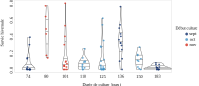
\includegraphics[width=1\linewidth]{survie-duree-deb-culture}
				\caption[Survie efficace du nématode.]{Survie hivernale du nématode ($\phi_h$) en fonction de  la durée 
				de la culture d'hiver et du mois de mise en place de la culture d'hiver. 
				Les barres horizontales au niveau des violin plots ont été dessinés pour indiquer
		        la médiane (ligne épaisse), les premier et troisième quartiles (lignes fines).}
		       \label{fig1:duree_pl} 
	      \end{figure}

			 
	      \begin{figure}
			  \centering
	           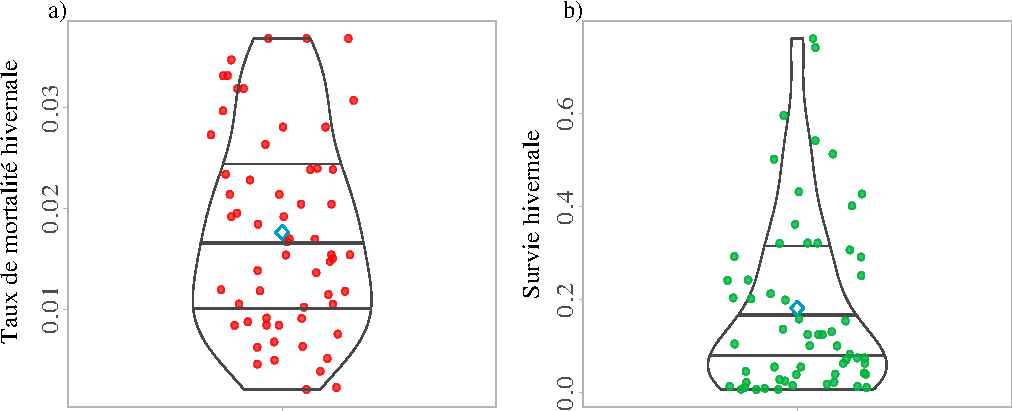
\includegraphics[width=1\linewidth]{survie_mortalite.pdf}
		      	\caption[a) Estimation du taux de mortalité du nématode  et b) survie des nématodes à intersaison]{a) 
		      	Estimation du taux de mortalité du nématode par jour. b) Survie des nématodes à intersaison obtenue à 
		      	l'aide de l'équation \eqref{survie_inter} . Le losange bleu représente la moyenne.  Les barres 
		      	horizontales au niveau des  violin plots ont été dessinés pour indiquer
	            la médiane (ligne épaisse), les premier et troisième quartiles (lignes fines).}
	            \label{fig2:survie_mort} 
		  \end{figure}
		
		
	 Dans cette section, le paramètre $\varphi$ a été estimé pour une  durée d'intersaison moyenne et à partir d'une estimation d'un taux de mortalité hivernal du nématode  en présence de salades sensibles ou plantes mauvais-hôtes qui sont souvent utilisées en rotation avec des tomates dans les systèmes de culture maraîchers \citep{Djian-Caporalino2019}. Cette étude nous a permis non seulement  d'avoir une meilleure idée de l'estimation de référence  de la survie à l'intersaison mais également de gammes de valeurs plus représentatives de la survie  du nématode adaptées pour des séquences de rotations de culture de tomates. Cette estimation de la probabilité de survie des nématode entre deux saisons de cultures  par l'utilisation des données terrain incluant  des  situations épidémiologiques pertinentes permet d'affiner nos prédictions et de mieux évaluer l'utilisation des rotations de culture  pour  la gestion des nématodes à galles des racines. Notons  que notre modèle complet, utilisé dans cette thèse dans un contexte bien spécifique peut s'appliquer à une large gamme de pathosystèmes pendant les saisons  mais également s'adapter très facilement à différentes situations épidémiologiques entre les saisons grâce à une ré-estimation de $\varphi$ selon la présence d'une culture (ou non) donnée et la durée de l'intersaison.
	 
	Notons que dans le chapitre~\ref{article} nous avons pris comme valeur de référence $\varphi = 0,4$ plutôt que $\varphi = 0,19$ pour effectuer notre modélisation. Ceci peut s'expliquer tout d'abord par le fait que la durée entre deux saisons de cultures prise dans notre modélisation et celle prise pour estimer le paramètre $\varphi$ à partir des données pluriannuelles de \gls{GEDUNEM} sont différentes. Pour effectuer l'estimation de $\varphi$ nous avons obtenu à partir des données terrain \gls{GEDUNEM} une valeur moyenne d'intersaison hivernale égale à 135 jours. Toutefois, pour notre modélisation nous avions une durée d'intersaison plus grande (de l'ordre de 200 jours).  De ce fait, pour une durée d'intersaison plus grande  nous supposons qu'une multiplication des nématodes à la fin de cette durée d'intersaison (notamment si les conditions climatiques s'améliorent à la fin de l'hiver)  aurait conduit à une survie plus élevée.
	
	Ensuite, nous avons montré dans l'analyse de sensibilité  pour une variation de $\pm{30}$ \% de ce paramètre autour de sa valeur de référence qu'il influence peu le rendement des cultures dans les rotations sur le long terme (voir \Cref{ans}). Enfin dans une étude ultérieure, suite à l'acquisition de ces nouvelles informations, nous avons pu démontrer  que la survie du nématode dans des gammes de valeurs se situant entre  10 et 52 \%  influence peu la durabilité des résistances par rapport aux scénarios épidémiologiques et au coût de fitness  (\autoref{survie_annexe}).  %Autrement dit, la variabilité de ce paramètre pour une gamme réaliste de survie du nématode entre les saisons n'aurait pas de conséquences très importantes pour les prédictions.
Cependant, on a constaté par le bais de notre modélisation qu'une survie très faible en moyenne (proche de  1 à 5 \%)  grâce à l'utilisation de traitements à l'intersaison, telles la solarisation et l'utilisation de plantes pièges pour éviter la multiplication de nématodes, pourraient améliorer la durabilité et protéger les résistances facilement contournables.	
	  
